% 2021-11-20
\begin{exercise}
      {ID-e7c1271a6b50a1f1dbded1e6e5ac717d7471a3b2}
      {Unvollständig}
  \ifproblem\problem\par
    % <PROBLEM>
    Gegeben ist folgendes unvollständige
    Prozessdiagramm:
    \begin{center}
      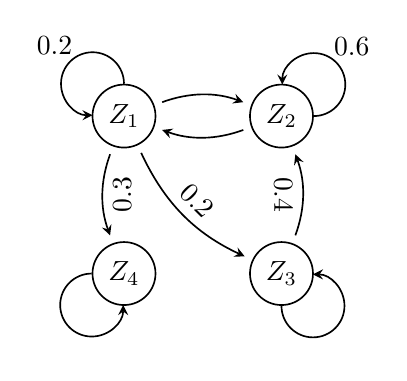
\begin{tikzpicture}[line width=0.6pt]
        \node[shape=circle,
              minimum size=8mm,
              inner sep=0pt,
              draw=black] (Z1) at (0, 2) {$Z_1$};
        \node[shape=circle,
              minimum size=8mm,
              inner sep=0pt,
              draw=black] (Z2) at (2, 2) {$Z_2$};
        \node[shape=circle,
              minimum size=8mm,
              inner sep=0pt,
              draw=black] (Z3) at (2, 0) {$Z_3$};
        \node[shape=circle,
              minimum size=8mm,
              inner sep=0pt,
              draw=black] (Z4) at (0, 0) {$Z_4$};
        %<OCTAVE>
        \draw[->, >=stealth] (Z1.90.000)
              arc[start angle=0.000,
                  end angle=270.000,
                  radius=4.000mm]
              node[pos=0.5,
                   shift={(135.000:8pt)}]
                   {\num{0.2}};
        %</OCTAVE>
        %myselfconnect("Z1", 135);
        %<OCTAVE>
        \draw[->, >=stealth] (Z2.0.000)
              arc[start angle=270.000,
                  end angle=540.000,
                  radius=4.000mm]
              node[pos=0.5,
                   shift={(45.000:8pt)}]
                   {\num{0.6}};
        %</OCTAVE>
        %myselfconnect("Z2", 45);
        %<OCTAVE>
        \draw[->, >=stealth] (Z3.270.000)
              arc[start angle=180.000,
                  end angle=450.000,
                  radius=4.000mm]
              node[pos=0.5,
                   shift={(315.000:8pt)}]
                   {\relax};
        %</OCTAVE>
        %myselfconnect("Z3", 315);
        %<OCTAVE>
        \draw[->, >=stealth] (Z4.180.000)
              arc[start angle=90.000,
                  end angle=360.000,
                  radius=4.000mm]
              node[pos=0.5,
                   shift={(225.000:8pt)}]
                   {\relax};
        %</OCTAVE>
        %myselfconnect("Z4", 225);
        \begin{scope}[->, >=stealth, shorten <=3pt, shorten >=3pt]
          \draw (Z1.20) to[out=20, in=160] node {}
                (Z2.160);
          \draw (Z1.295) to[out=295, in=155]
                         node[rotate=-45, above] {\num{0.2}}
                (Z3.155);
          \draw (Z1.250) to[out=250, in=110]
                         node[rotate=90, below] {\num{0.3}}
                (Z4.110);
          \draw (Z2.200) to[out=200, in=340] node {}
                (Z1.340);
          \draw (Z3.70) to[out=70, in=290]
                        node[rotate=-90, below] {\num{0.4}}
                (Z2.290);
        \end{scope}
      \end{tikzpicture}
    \end{center}
    \begin{enumerate}[a)]
      \item Vervollständigen Sie das Prozessdiagramm
            und geben Sie die Übergangsmatrix an.
            Wie nennt man den Zustand $Z_4$?
      \item Sie befinden sich anfangs mit jeweils
            \SI{50}{\percent} Wahrscheinlichkeit
            in Zustand $Z_1$ bzw. Zustand $Z_2$.
            Geben Sie die Startverteilung als
            Vektor an.
      \item Sie multiplizieren die Übergansmatrix mit
            der Startverteilung. Interpretieren Sie
            den Wert in der zweiten Zeile des
            Ergebnisvektors.
      \item Berechnen Sie die Zustandsverteilung nach
            zwei Schritten.
    \end{enumerate}
    % </PROBLEM>
  \fi
  %\ifoutline\outline\par
    % <OUTLINE>
    % </OUTLINE>
  %\fi
  %\ifoutcome\outcome\par
    % <OUTCOME>
    % </OUTCOME>
  %\fi
\end{exercise}
